\documentclass{article}

% Language setting
% Replace `english' with e.g. `spanish' to change the document language
\usepackage[english]{babel}

% Set page size and margins
% Replace `letterpaper' with`a4paper' for UK/EU standard size
\usepackage[a4paper,top=2cm,bottom=2cm,left=3cm,right=3cm,marginparwidth=1.75cm]{geometry}

% Useful packages
\usepackage{amsmath}
\usepackage{graphicx}
\usepackage{listings}
\usepackage{xcolor}
\usepackage[colorlinks=true, allcolors=blue]{hyperref}

\usepackage{algorithm, algpseudocode}
\usepackage{csquotes}
\usepackage{subfig}

\definecolor{codegreen}{rgb}{0,0.6,0}
\definecolor{codegray}{rgb}{0.5,0.5,0.5}
\definecolor{codepurple}{rgb}{0.58,0,0.82}
\definecolor{backcolour}{rgb}{0.95,0.95,0.92}

\lstdefinestyle{mystyle}{
    backgroundcolor=\color{backcolour},   
    commentstyle=\color{codegreen},
    keywordstyle=\color{magenta},
    numberstyle=\tiny\color{codegray},
    stringstyle=\color{codepurple},
    basicstyle=\ttfamily\footnotesize,
    breakatwhitespace=false,         
    breaklines=true,                 
    captionpos=b,                    
    keepspaces=true,                 
    numbers=left,                    
    numbersep=5pt,                  
    showspaces=false,                
    showstringspaces=false,
    showtabs=false,                  
    tabsize=2
}

\lstset{style=mystyle}
\newcommand{\code}[1]{\lstinline|#1|}

\title{Homework 4\\CS3316 Reinforce learning}
\author{Ng Tze Kean\\Student number: 721370290002}

\begin{document}
\maketitle

\begin{titlepage}
\end{titlepage}

\section*{Architecture and usage}

In this experiment we create classes of deep Q networks (DQN) instead and train them
on the MountainCar environment from OpenAI gym. We test 4 variations of DQN
in this experiment as an improvement to the classical DQN implementation. The
variations being Double-DQN, Dueling-DQN, Double-Dueling-DQN and Experienced
Replay DQN. Base
classes are also built to support the DQN learning, mainly Replay memory and the
SumTree class to support the replay memory.

The classes below are the classes that are constructed which one can use to run
the experiment on.

\begin{lstlisting}[language=python]
    DQN()
    DoubleDQN()
    DuelingDQN()
    DoubleDuelingDQN()
    PrioritizedDQN()
\end{lstlisting}

We can view the code, specifically the function \code{train}. We can modify
the agent class in the method to call the specific agent that you want to run
the experiment on. The agent will then be trained on the environment and the
results will be plotted on the graph.

\begin{lstlisting}[language=python]
    def train():
    env = gym.make("MountainCar-v0")
    n_episodes = 500
    env = gym.wrappers.RecordEpisodeStatistics(env, deque_size=n_episodes)
    
    agent = DoubleDuelingDQN(env.observation_space.shape[0], env.action_space.n)
\end{lstlisting}

\section*{Classical DQN}

We implement the classical DQN from the pseduocode given

\begin{algorithm}
    \caption{deep Q-learning with experience replay}\label{alg:cap}
    \begin{algorithmic}
    \State Initialize replay memory D to capacity N
    \State Initialize action-value function Q with random weights $\theta$
    \State Initialize target action-value function $\hat Q$ with weights $\theta^- = \theta$
    \For{$episode = 1, M$}
        \State Initialize sequence $s_1 = {x_1}$ and preprocessed sequence $\phi_1 = \phi(s_1)$
        \For{$t=1,T$}
        \State With probability e select a random action $a_t$
        \State otherwise select $a_t = \arg \max_a Q()$
        \State Execute action at in emulator and observe reward $r_t$ and image $x_{t+1}$
        \State Set $s tz1~s t ,at ,xtz1$ and preprocess $\phi_{t+1} = \phi(s_{t+1})$
        \State Store transition $(\phi_t,a_t,r_t,\phi_{t+1})$ in D
        \State Sample random minibatch of transitions $(\phi_j,a_j),r_j$ from D
        \State $y_j = $
        \State Perform a gradient descent step on $(y_j - Q(\phi_j,a_j,\theta))^2$ with respect to the
        \State network parameters $\theta$
        \State Every C steps reset $\hat Q = Q$
        \EndFor
    \EndFor
    \end{algorithmic}
\end{algorithm}

We note that there are 2 components to the classical DQN implementation. We will
go through in detail the 2 and how it is implemented in our experiment.

\subsection*{Experience replay}
The idea behind this concept is that instead of training on a state, action pair
and discarding the sample, we will instead store this sample in a buffer which
will contain the experience of the agent. In our implementation, the class providing
this storage is the \code{ReplayMemory} which stores objects of \code{Transition}.

\begin{displayquote}
    Initialize replay memory D to capacity N
\end{displayquote}

We will then replay these memory through random sampling from the buffer. This
allows for elimination of correlation when we train on experience that occurs in
sequence. The model would then be able to learn the actions that lead to learning
actions that truely lead to a higher Q-value.

\subsection*{Fixed Q target}

When we compute the TD error, we calculate the difference between the TD target
and the and the current Q value. However, we do not know the actual TD target, so
through the bellman equation we estiamte the TD target as the reward of taking
that action at that state plus the discounted highest Q value for the next state.

We now realism that the same parameters are also used to compute the current Q
value, leading to a high correlation between the 2 variables. Thus, each time we
modify weights, the TD target shifts, leading to an oscillation of the 2 values.

\begin{displayquote}
    Initialize action-value function Q with random weights $\theta$
    Initialize target action-value function $\hat Q$ with weights $\theta^- = \theta$
\end{displayquote}

To handle this issue, we introduce 2 networks a policy and target network for
stability. The target network will be lagging behind the policy network in its
updates to its weights, but this will fix the Q target allowing for the network
to achieve greater stability.

\section*{Improvements}

We look at 2 improvements that we made to the classical agent.

\subsection*{Double DQN}

The implementation of Double DQN aims to tackle the overestimation of Q values
during training. The issue with the computation of the TD target is that we cannot
be sure that the best action for the next state is the action that gives the max
Q value.

The question is made clearer by realizing that the Q value is dependent on actions
that have been taken and the neighboring states that have been explored. For agents
that do not have enough experience, the Q value is noisy and the current best action
may not be the global best action. Thus, we see an issue of having non-optimal actions
being learnt as the optimal action.

\begin{lstlisting}[language=python]
    state_action_values = self.policy_net(state_batch).gather(1, action_batch) # Q(s,a)

    next_state_values = torch.zeros(DQN.BATCH_SIZE, device=device)
    max_action = self.policy_net(non_final_next_states).max(1).indices.view(-1, 1)
    with torch.no_grad():
        next_state_values[non_final_mask] = self.target_net(non_final_next_states).gather(1, max_action).flatten()
    # Compute the expected Q values
    expected_state_action_values = (next_state_values * DQN.GAMMA) + reward_batch

    loss = self.loss_func(state_action_values, expected_state_action_values.unsqueeze(1))
\end{lstlisting}

To tackle this issue, we use 2 network to separate the selection of action from
the generation of the TD target. We can use the policy network to select the best
action, the argmax Q(s,a), and the target network to calculate the Q value of taking
this action in the next state. This will decouple the action selection and TD target
generation, leading to a reduction in overestimation of Q values.

\subsection*{Dueling DQN}

Also known as DDQN. This is based off the idea that Q value is made of 2 components
the state and action. The value of being in a state and the action that gives rise
to the highest value. We can try to define the following

\[
    Q(s,a) = A(s,a) + V(s)
\]

Thus, we would have a common layer that takes in the input and 2 separate layers
that aim to predict (1) state value V and (2) advantage of actions. An aggregation
layer will then be used to combine the 2 layers.

\begin{lstlisting}[language=python]
    def forward(self, x):
        A = self.A_head(F.relu(self.fc1(x)))
        V = self.V_head(F.relu(self.fc1(x)))
        Q = V + A - A.mean(1).view(-1, 1)  # Q(s,a)=V(s)+A(s,a)-mean(A(s,a))
        return Q
\end{lstlisting}

By decoupling the estimation, intuitively our DDQN can learn which states are
valuable without having to learn the effect of each action at each state
since it is also computing V(s) through a separate layer. Then, the advantage
that we get is that for states where their actions do not affect the environment
in a relevant way, the agent need not calculate the value of each action for the
state.

In our case where the world is continuous, this could be useful as it eliminates
states that are not relevant to reaching the goal, allowing the agent to quickly
converge to optimal.

\subsection*{Combining the 2 improvement}

We finally combine the 2 improvements into a single agent to see how it improves
and how it might perform in an environment where positive rewards are extremely
sparse.

\subsection*{Prioritized experience replay}

We also search the internet for the implementation of the prioritized experience
replay. The idea behind this is that not all experiences are equal. Some experiences
are more important than others and should be sampled more frequently. The idea
is to assign a priority to each experience and sample based on the priority.

We use a sumtree as the data structure to store the experiences. The sumtree is
a binary tree where the parent node is the sum of the children. The sumtree allows
us to sample efficiently based on the priority of the experience.

\section*{Results}

We begin first with the simple DQN and we can see that the agent performs very
poorly over 100 episodes. We see a lot of fluctuations and swings in the model's
performance. We also note that due to the limitations of time, we fixed the
hyperparameter of the agents. The agents will be tested over 500 episodes with the
following parameters.

\begin{lstlisting}[language=python]
    learning_rate: float = 0.0005
    total_length_memory: int = 2000
    train_start_length_memory: int = 100
    updating_batch_size: int = 64
    discount_factor: float = 0.98
    target_update_interval: int = 10
    epsilon_start: float = 1.0
    epsilon_decay: int = 20000
    epsilon_end: float = 0.05
\end{lstlisting}

\begin{figure}[h]
    \centering
    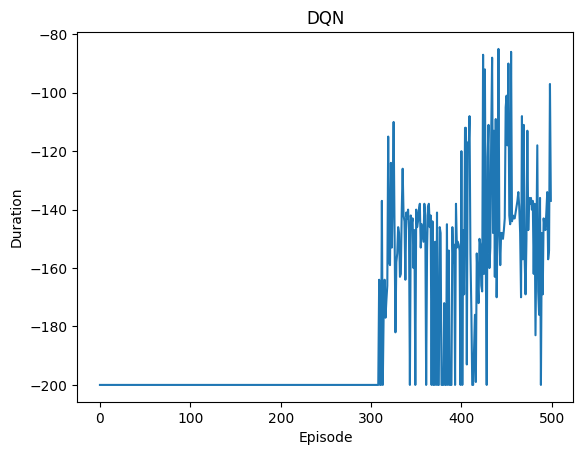
\includegraphics[width=0.6\textwidth]{dqn.png}
    \caption{Parameters to achieve optimal path}
\end{figure}

\newpage

Moving on to the improved methods, we have double DQN and dueling DQN which has
performed significantly much better than the base DQN model. The parameters of
the agents are kept the same and the only difference is the agent the techniques
described above.

\begin{figure}[h]%
    \centering
    \subfloat[\centering Double DQN]{{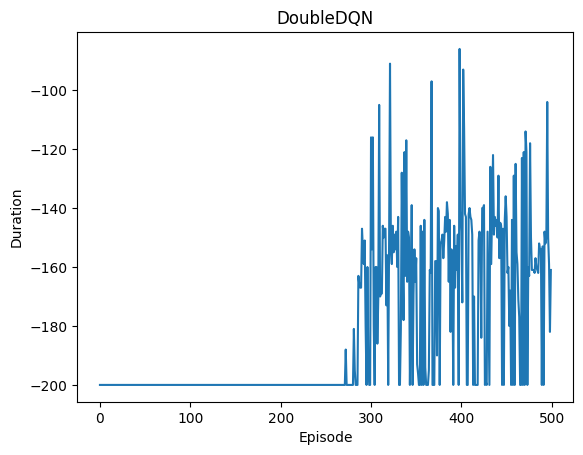
\includegraphics[width=6cm]{double.png} }}%
    \qquad
    \subfloat[\centering Dueling DQN]{{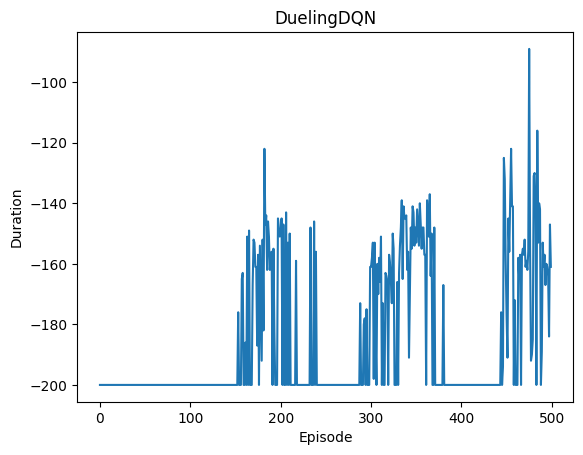
\includegraphics[width=6cm]{dueling.png} }}%
    \caption{Implementation of both algorithm}%
    \label{fig:example}%
\end{figure}

We try to also experiment how the agent would be different if we were to combine 
these 2 methods. We are interested to find out if the 2 techniques can
synergise with each other, or they would cause conflicts in the learning. We create
a combined class \code{DoubleDuelingDQN} which inherits from both classes.

\begin{figure}[h]
    \centering
    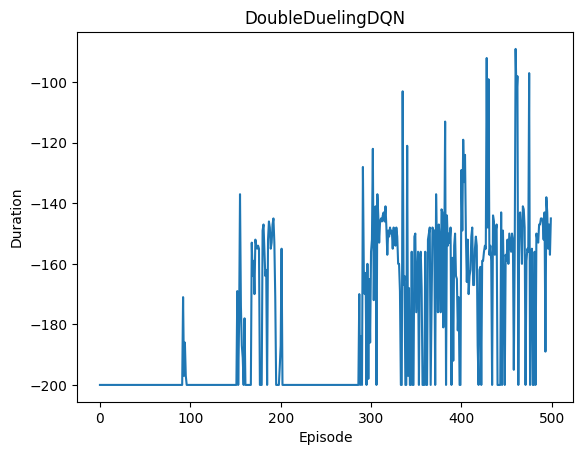
\includegraphics[width=0.6\textwidth]{double_dueling.png}
    \caption{Double dueling agent combined performance}
\end{figure}

\newpage

The final agent that we have implemented is the prioritized experience replay with
double DQN. We can see that from all the runs, this agent performs the best
and has the most stable learning curve.

This is probably because the algorithm would choose the best episodes to cache.
The episodes are then selected based on the temporal difference, that is the episodes
that would bring the greatest difference to the Q value.
The specific selection of episodes would help the agent to convert in a
faster manner with less noise.

\begin{figure}[h]
    \centering
    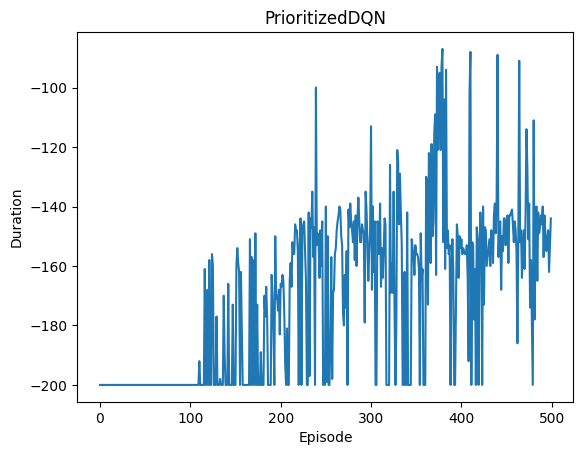
\includegraphics[width=0.6\textwidth]{prioritised_experience.png}
    \caption{Prioritized experience replay with double DQN performance}
\end{figure}

\end{document}